\subsection{Product Perspective}
\subsubsection{Scenarios}
\begin{enumerate}
    \item \textbf{Educator creates a tournament} \newline Professor Emanuelle, a computer science educator giving "Introduction to Programming" course in Politecnico di Milano, decides to improve her student's understanding about programming through coding exercises. She is already registered in CodeKataBattle as educator, so she logs in the platform by his credentials, which are email and password. Then, she clicks the "Create Tournament" and a form screen is prompted. She fills out the form respectively: \newline
    - entering tournament title, "Winter Semester Coding Exercise 1", \newline
    - adding description of the tournament, \newline
    - choosing a deadline for subscription. After clicking "Next" button\newline
    Professor Emanuelle is asked to select colleagues for permission to create battles in this tournament. She selects 2 of her colleagues because they all together gives the same lecture. Finally, she clicks on "Create" button and tournament is created. She is directed to "My tournaments" sections after creation.
    \item \textbf{Student Registers for tournament} \newline Emre is a Bachelor student in Computer Science in Politecnico di Milano. At the start of the winter semester he registered CodeKataBattle as a requirement of his "Introduction to Programming" course. In the middle of semester, he gets email notification about a tournament created by Professor Emanuelle in the platform. Then, He clicks the link in email. Because he has already logged in platform with his email and password, he is redirected to tournament's page, where he finds detailed information about Emanuelle's tournament. After reading description, he thinks that this tournament will be very helpful for him to understand the topics covered in the lecture. So he clicks to "Register" button to enroll tournament. Some registration details consisting of description, educators, and tournament creator are shown in screen. Also he is informed that he will get email notifications about upcoming battles, battle and tournament rankings. Finally, Emre clicks on "Accept and Register" button and registers the tournament.
    \item \textbf{Educator Sets Up a Battle} \newline A week ago Professor Mottola, was invited to tournament created by his colleague in the CodeKataBattle platform. He accepted the invitation and learned about the tournament from its description. He also gives "Introduction to Programming" course and want to to create a new exercise about the topic he showed in the last lecture, which is "Recursion". After subscription deadline passed, he logged back into CKB, he selects the "Create Battle" option within the "Winter Semester Coding Exercise 1" tournament. He is presented with a detailed form where he inputs the battle's title, "Check if String is Palindrome" and provides a thorough description that includes the battle's focus on recursion, expected coding languages (Java and Python, both accepted) and software project including necessary scripts for build automation (Gradle for Java, no need for Python) and test cases. To encourage collaboration, he sets the minimum and maximum group size to three and five students, respectively. he then specifies the registration deadline, two weeks from the current date, and a final submission deadline, giving students a month to work on their solutions. Finally, he configures additional scoring parameters as \textbf{efficiency}, choosing from a list of aspects including reliability, maintainability, etc. Then he clicks on "Create" button and he is redirected to battle main page illustrating information about battle. After a couple of minutes, he got an email saying that an email about this battle are sent to all students in the tournament.\newline \newline
    \item \textbf{Student Joins for Battle} \newline Samet got a notification from the tournament he enrolled saying that Professor Mottola has created a battle with name "Check if String is Palindrome". He clicks on link, and reads the description carefully. He clicks on "Register" button then a screen is shown asking Samet whether he wants to invite other students to form a team or not. Samet selects "Yes", then, he names her team 'Code Warriors' as a first step.Then he chooses students from a list of students registered to tournament, considering minimum and maximum group size. Samet knows Emre, Jack and Luca also registered to tournament, so sends them invitations. After clicking "Complete", he is redirected to battle information page. In this page there is a section showing group status, which is pending until all invitations are answered. After a while, Samet sees that Emre and Luca accepted but Jack rejected. Because minimum group size is fulfilled, Samet clicks on the "Finalize" button indicating final decision. Thanks to the help of instructions during the process, Samet understands that if he wants to decline registration, he should have clicked on "Decline" button. After every member accepted invitation finalize registration, process ends and status become "Registered". They are given a competitor id.
    \item \textbf{Students Sets Up Environment for CodeKataBattle} \newline With the 'Code Warriors' team formed and the registration deadline for the "Check if String is Palindrome" battle passed, the CKB platform takes its next automated step. It creates a unique GitHub repository for the battle, containing the provided code kata with its test cases and build scripts. The system then sends an email to Emre, Samet, and Luca with the repository link and instructions. The team members collaboratively decide to schedule a virtual meeting to set up their working environment. During the meeting, they fork the repository to their group account and set up GitHub Actions in order to make proper API calls with competitor id they have. This setup is crucial for automating their workflow and ensuring that every code push not only updates their repository but also notifies the CKB platform. They test the setup by pushing a minor change, and upon seeing that the CKB platform acknowledges their commit, they know their system is correctly configured. This marks the start of their coding journey in the battle.
    \item \textbf{Students Solve Battle Challenge} \newline After forking the project and setting environment, they started to think about the solution of project. As they understand from description they should return "True" or "False" regarding whether the given string is a palindrome. They implement algorithm and commit/push the code to the repository. Each push prompts the platform to pull the latest code, run tests, and analyze the quality of their solutions using static analysis tools. After a while, they revisit the ranking in the battle's page to see their score of last push. They see their scores in 3 different category: \newline
    - functional aspects: 32/80 (4/10 test cases passed) \newline
    - timeliness: 5/5 \newline
    - quality level of the sources: 8/10 (Aspects: Efficiency) \newline
    In the rankings they are informed via tool tips about the scaling of scores and calculation methods of them. So they decides to focus on more on code and tries to find why some test cases are not passed. The team keeps an eye on the CKB dashboard, which updates their battle score after each commit. They note improvements in their score as they refine their solutions, ensuring more test cases pass and optimizing their code for better quality. This iterative process of coding, committing, and refining continues, with the team members frequently discussing strategies and sharing insights to improve their solutions. After looking some exercises related to recursions they finally finds the wrong part in the algorithm they implemented. After changes they commit and push the code. They sees in the rankings that they got 93 points from battle. This iterative process of coding, committing, and refining continues, with the team members frequently discussing strategies and sharing insights to improve their solutions.They thinks that this is most efficient algorithm they can implement. So they decides not to do anything else until koda battle deadline. \newline
    \item \textbf{Educator Evaluates Submission Manually} \newline
    After submission deadline expires, there is a consolidation stage enabling educators to assign optional points for teams. Professor Mottola begins her manual evaluation of the submissions for the "Check if String is Palindrome" battle. He logs into CKB and accesses the educator's dashboard from the battle's page, where he can review each team's submission. In this page code of the submission and other materials from the repository are shown to the educator. He starts from latest submission and gives extra points if he finds solution by analyzing 'Code Warriors', impressed by their timely submission and high score, viewable in rankings table. Professor Mottola examines their code, focusing on the efficiency of their solution, which got 8/10 from analysis tool. Considering these factors, she awards them a high personal score. This score reflects her assessment of their problem-solving skills and coding proficiency, adding a crucial human element to the automated evaluation. 
    \item \textbf{Educators Analyze Tournament Leaderbord} \newline
    Professor Emanuelle have created a tournament called as "Winter Semester Coding Exercise 1" at the begining of the semester. Some other colleagues of her registered the tournament as educators and created koda battles during semester. During semester, she has viewed the leaderboard and at the end of every week she has exported the result. Eventually, at the end of the semester Professor Emanuelle closes the tournament. She then goes to leaderboard screen and started to see general success of her students by comparing leaderboard exports from the very first battle. In this way she notices that leaderboard becomes more comptetitive as we get closer to the end of the year. She interpret this situation as students improved their programming skills battle by battle. After analyzing the leaderboard she searches another ongoing tournaments of another professors from university to see success of their students on different tournaments created by teachers of different courses.
    
\end{enumerate}
\newpage
\subsubsection{Domain Class Diagram}
In Figure(1.1), the Domain Class Diagram for the CodeKataBattle (CKB) platform is illustrated. This diagram is a crucial element in understanding the structure and relationships within the CKB system. It visually represents the key classes, their attributes, and the interactions among them in the context of the platform. This diagram is designed to provide a clear and concise overview of the domain model, offering insights into how the different components of the CKB platform interact to facilitate a competitive and educational coding environment. Below are descriptions of the most relevant parts of the diagram:
\begin{itemize}
    \item \textbf{Student and Educator Classes}: The diagram differentiates between two primary types of Users: students and educators. Both share common attributes such as name, surname, email and password, but they interact with the system differently. Educators, for instance, have the ability to create tournaments and battles, while students can participate in these competitions.
    \item \textbf{Tournament and Battle Classes}: These classes represent the core competitive elements of CKB. A Tournament, created by an Educator, can contain multiple Battles. Each Battle, associated with a specific Tournament, includes attributes like description, start\_date, end\_date, min-max of group size and scoring\_criteria.
    \item \textbf{Competitor Class}: Reflecting the collaborative aspect of CKB, the Competitor class includes attributes like name and members, the latter being a collection of Students in case of team formation. If a student register individually, members field consists of just one member and name is student's name.
    \item \textbf{Submission Class}: This class represents the solutions submitted by Competitor for a Battle. Key attributes include code\_repository\_link, time\_of\_submission, and score.
    \item \textbf{GitHub Integration}: A separate class to represent the integration with GitHub, showing how students' code repositories are connected to the CKB platform for automatic evaluation. For every battle an instance of Github Integration is created and responsible for the API calls from Github Actions and pulling source code from forkedr repository.
    \item \textbf{Scoring Class}: This class illustrates the scoring mechanism of CKB, including both automated and manual scoring components as detailed in the project description.
\end{itemize}
\begin{center}
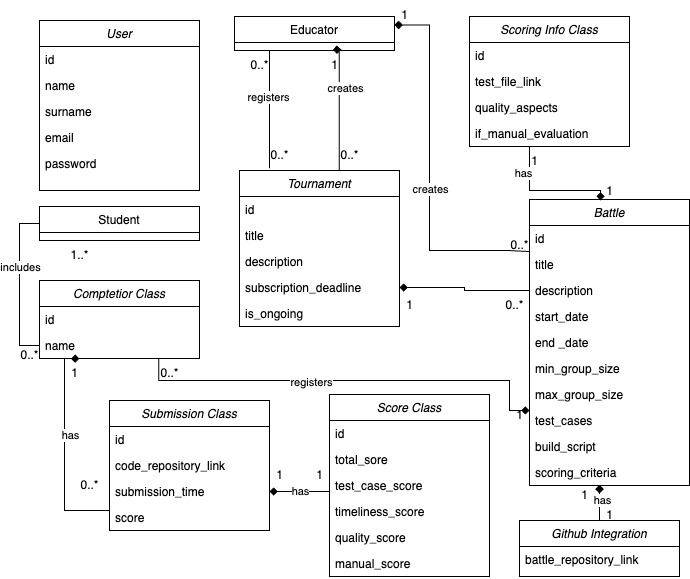
\includegraphics[width=\textwidth,height=\textheight,keepaspectratio]{DomainClassDiagramRASD (1).jpg}
\end{center}
\newpage
\subsubsection{Statecharts}
The statecharts presented in this section elucidate the operation of the CodeKataBattle (CKB) project, illustrating the state transitions for a code kata battle and a tournament within the platform. Especially for tournament, statechart is very crucial to gain a better understanding of the tournament.\newline
\textbf{Tournament}
\begin{center}
    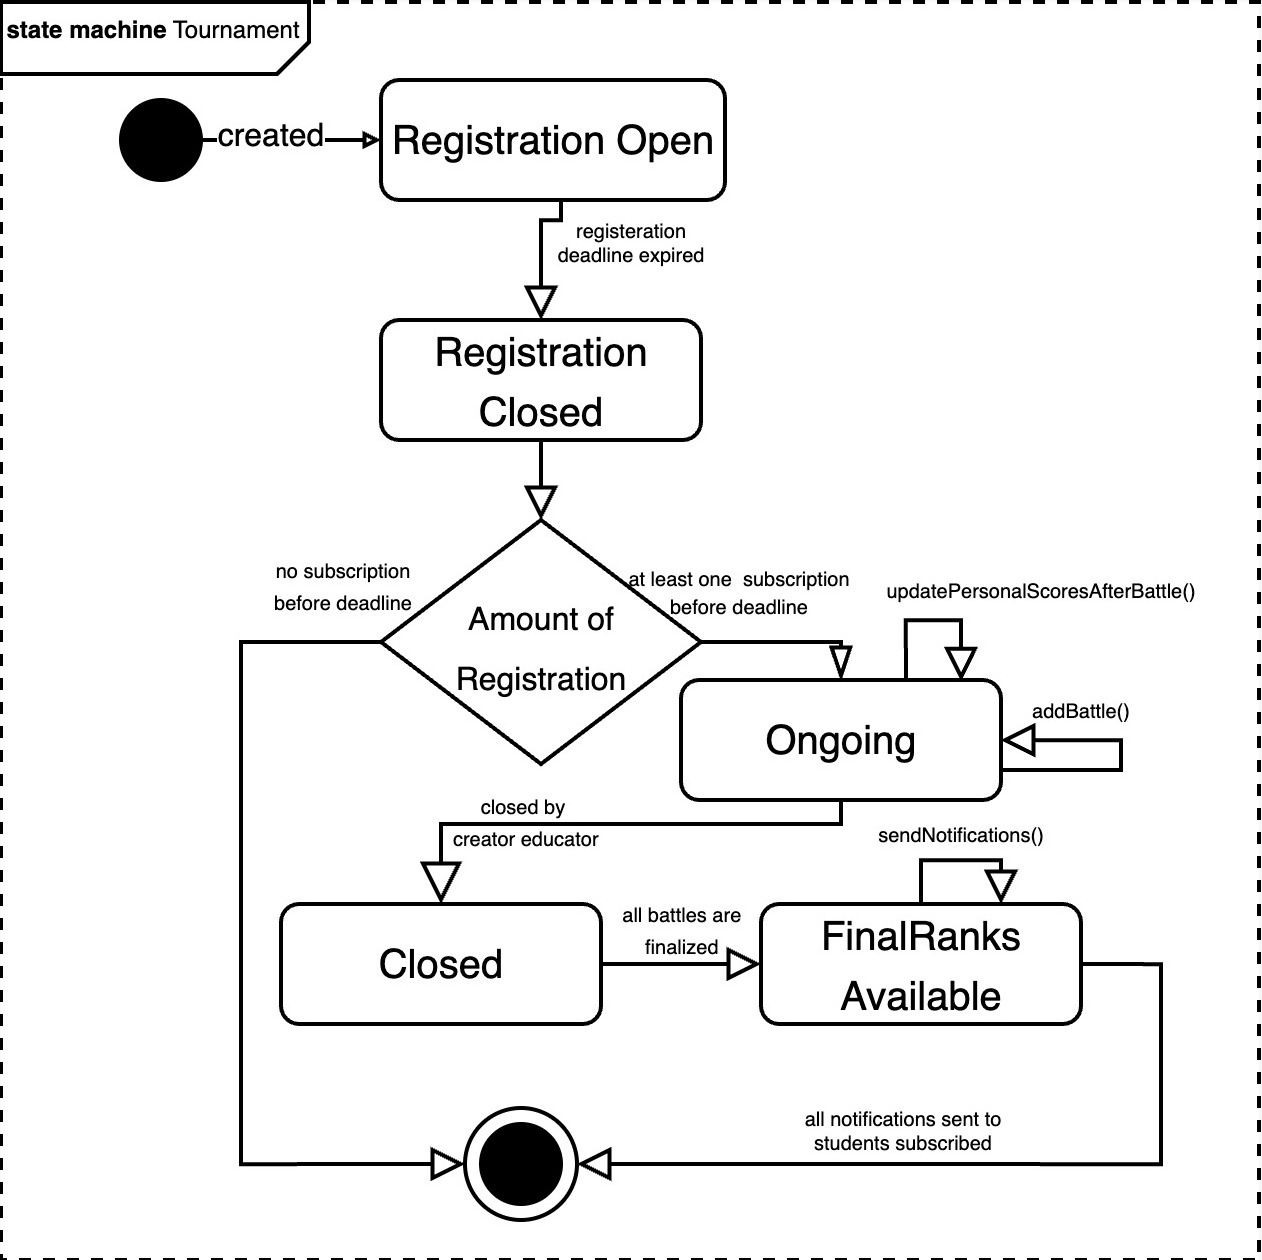
\includegraphics[scale=0.2]{Images/tournamentStatechart.jpeg}
\end{center}
Firstly, tournament is in the very first state called as "Registration Open", which is indicating that Tournament is created and registration is open for students and invited educators. Until the registration deadline they can register. When the deadline expired registration closed, so tournament goes into "Registration Closed" state. In this state, process controls the amount of registration for tournament. If there is no registration it goes to "Final" state. Otherwise tournament starts with "Ongoing" state. In this state, throughout the tournament, educators can create battles and personal scores are updated after every battle. If creator educator closes the tournament, it goes to "Closed" state. However, there can be some battles in consolidation stages and it is mandatory to finalize them to calculate final ranks. After all battles are finalized, the tournamnet transitions to "FinalRankAvailable" state in which notifications about final rankins are sent to the students. After finishing this notification process tournament reaches the "Final" state. There won't be any rank changes or notification hereafter. \newpage
\textbf{Battle}\newline
\begin{center}
    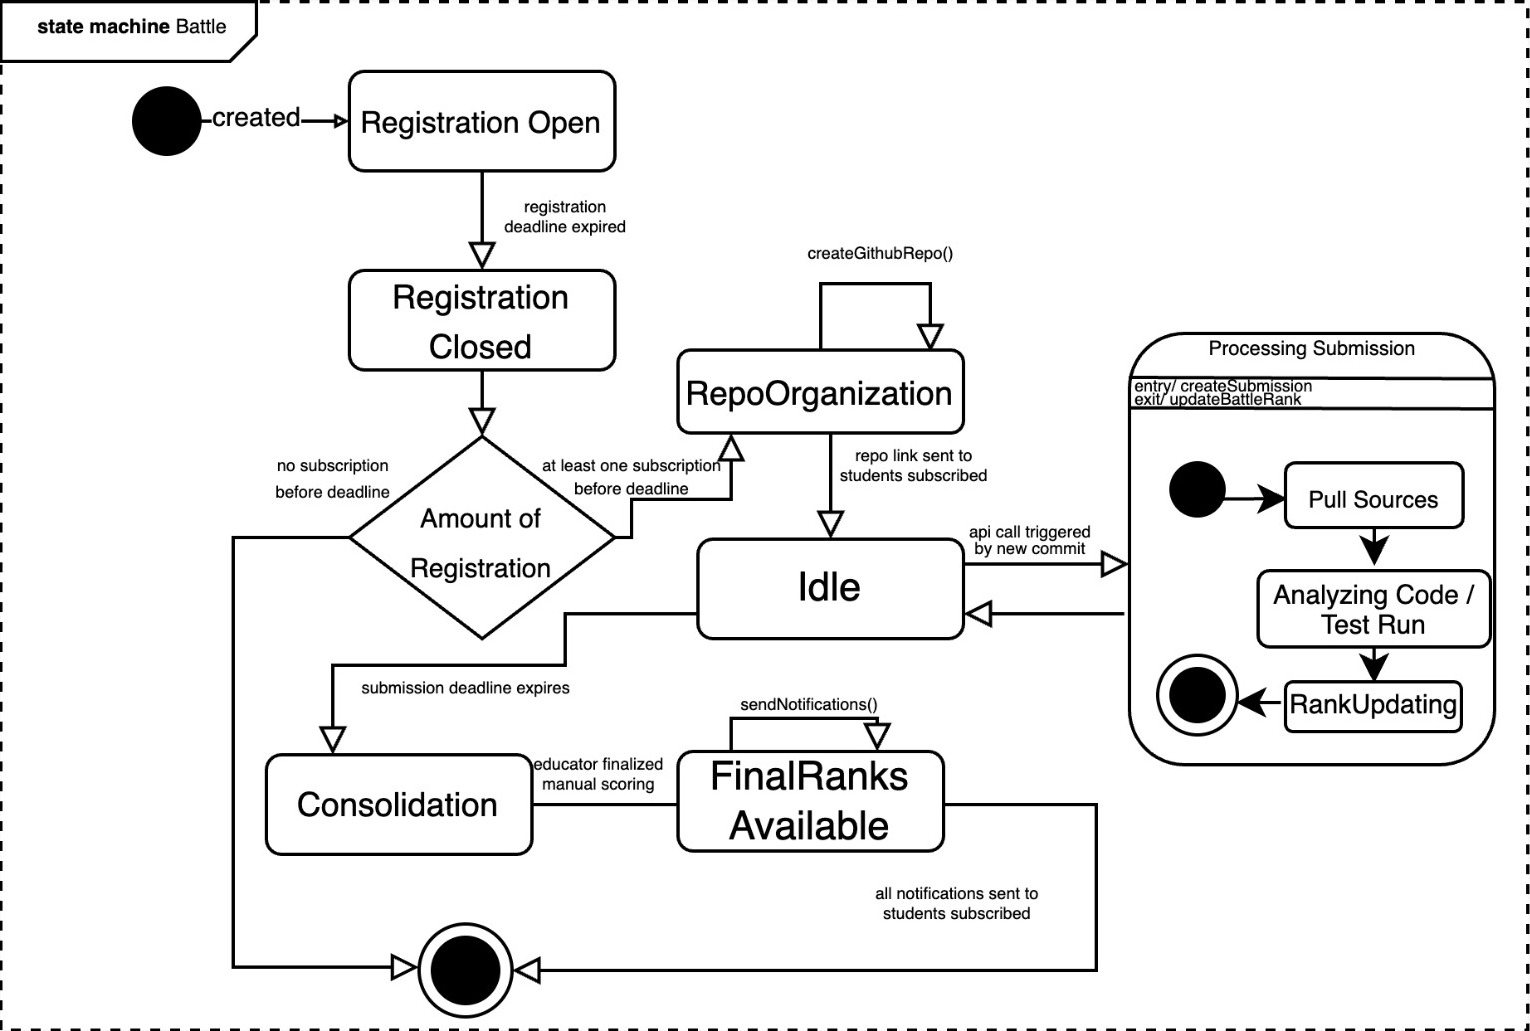
\includegraphics[scale=0.2]{Images/battleStatechart.jpeg}
\end{center}
Firstlyi tournament is created with "Registration Open" state. In this state, students cann register to battle with teams or individually. When the deadline expires, Battle goes into "Registration Closed" state. At this time, it is calculated that if there is any registration for battle. If no, it goes to "Final" state with no registration and any other action. If there is registrations, it goes to new state called as RepoOrganization in which Github repository for the battle is created with proper instructions.Sending link and instructions trigger the process to go into "Idle" state. This means that Battle has started and waits for API calls from forked repositories, triggered by a new commit. An API call from  repositories of competitor leads to go into "Processing Submission. Here with the "createSubmision" input 3 sequential states follow each other, respectively, "Pull Sources", "Analyzing Code / Test Run" and "RankUpdating". In this 3 state code is pulled and analyzed. ,then, score and rankings are updated.  Eventually, it returns to "Idle" state. Until submission deadline students' commit can change their score. When the deadline expires, Battle goes into "Consolidation Stage" state in which educators can change rankings via manual scorings. When they finalized, Battle is closed, indicating as state "FinalRanksAvailable". Immediately, notification sending process starts. After all notifications are sent, Battle goes into Final state.
\newpage
\subsection{Product Functions}
\subsubsection{User Authentication}
Login and Sign up functions is available for all kind of user. There is two type of user in the platform, which should be indicated when signing up to system. In signup all users are requested to provide the following information respectively:
name, surname, email, password and type. A verification email is sent to provided email in order to verify user. After confirmation, user is redirected to platform login page. Here, email and password is required to enter the platform. Also "stay logged in" option is available in order to avoid the need to enter credentials every time entering the platform.
\subsubsection{Tournament}
In the platform, educators can create tournament with a title, description and deadline for registration.  Title and description should briefly explain tournament content. Until the given subscription deadline, student can subscribe to the tournament. Also creator should be able to invite some of her/him colleagues to tournament in order to create battles in it. While tournament continues, educators creates battles that students can participate. Scores students gained from battles are summed up for the leaderbord of the tournament. After creator educator closes the tournament, if all battles are finalized, all scores from battles are summed up to build final leaderbord including rankings. In the period of tournament students are notified with emails about new battles. Also, at the end of the tournament, final rankings are sent to students.
\subsubsection{Battle}
An educator in a tournament can be able to create battles in it. This battles are created with title, description, start-end dates, min-max group sizes, test cases, build scripts and scoring criteria. Scoring criteria is defined by educator. It should provide system a test file including test cases, whether there is manual evaluation, and quality aspects chosen from a list in the system such as efficiency, clean code etc. With this information system can evaluate the submissions.

